\subsection{Разметка наборов данных}
    Для построения требуемого в работе набора данных необходимо найти множество связей твит-новость.
    Процесс поиска связей твит-новость называется \textit{разметкой набора данных}. В работе использовано два способа разметки:
    \begin{enumerate}
        \item автоматическая разметка набора данных;
        \item ручная разметка набора данных.
    \end{enumerate}

    В результате разметки получено большое количество пар твит-новость, в которых твит, практически полностью совпадает с заголовком новости.
    В дальнейшем, для удобства обозначение подобных пар, будем называть связь твит-новость \textit{тривиальной}, если в заголовке статьи встречается менее половины слов из твита.

    \subsubsection{Автоматическая разметка набора данных}
        Автоматически построенный набор данных состоит из всех собранных новостей и твитов, которые содержат ссылку на одну из собранных новостей.
        Автоматически разметив полученную информация, получили множество состоящее из 4324 твитов, 13711 новостей, а также 4324 связей между ними.

        Полученный набор данных был проанализирован, с целью выявления количества нетривиальных связей.
        Для каждого твита был взят его текст, для каждой новости~---~заголовок.
        Все полученные тексты поэтапно преобразованы согласно алгоритму, который сопоставляет тексту множество слов и состоит из следующей последовательность действий:
        \begin{enumerate}
            \item текст конвертируется в формат unicode;
            \item текст разбивается на токены;
            \item полученное множество токенов очищается от токенов, не являющихся словами;
            \item из множества удаляются все слова входящие в словарь стопслов;
            \item из множества удаляются все дубли.
        \end{enumerate}
        На основе предподготовленных данных для каждой пары твит, связанная с твитом новость измерялось две метрики:
        длина пересечения слов твита и слов новости, нормализованная по длине новости;
        количество слов в твите, которые не встречаются в новости.

        На рисунке~\ref{pic:auto_histogram} изображена зависимость количества пар твит-новость от длины пересечения слов твита и слов новости, нормализованной по длине новости.
        \begin{figure}[h!]
            \center
            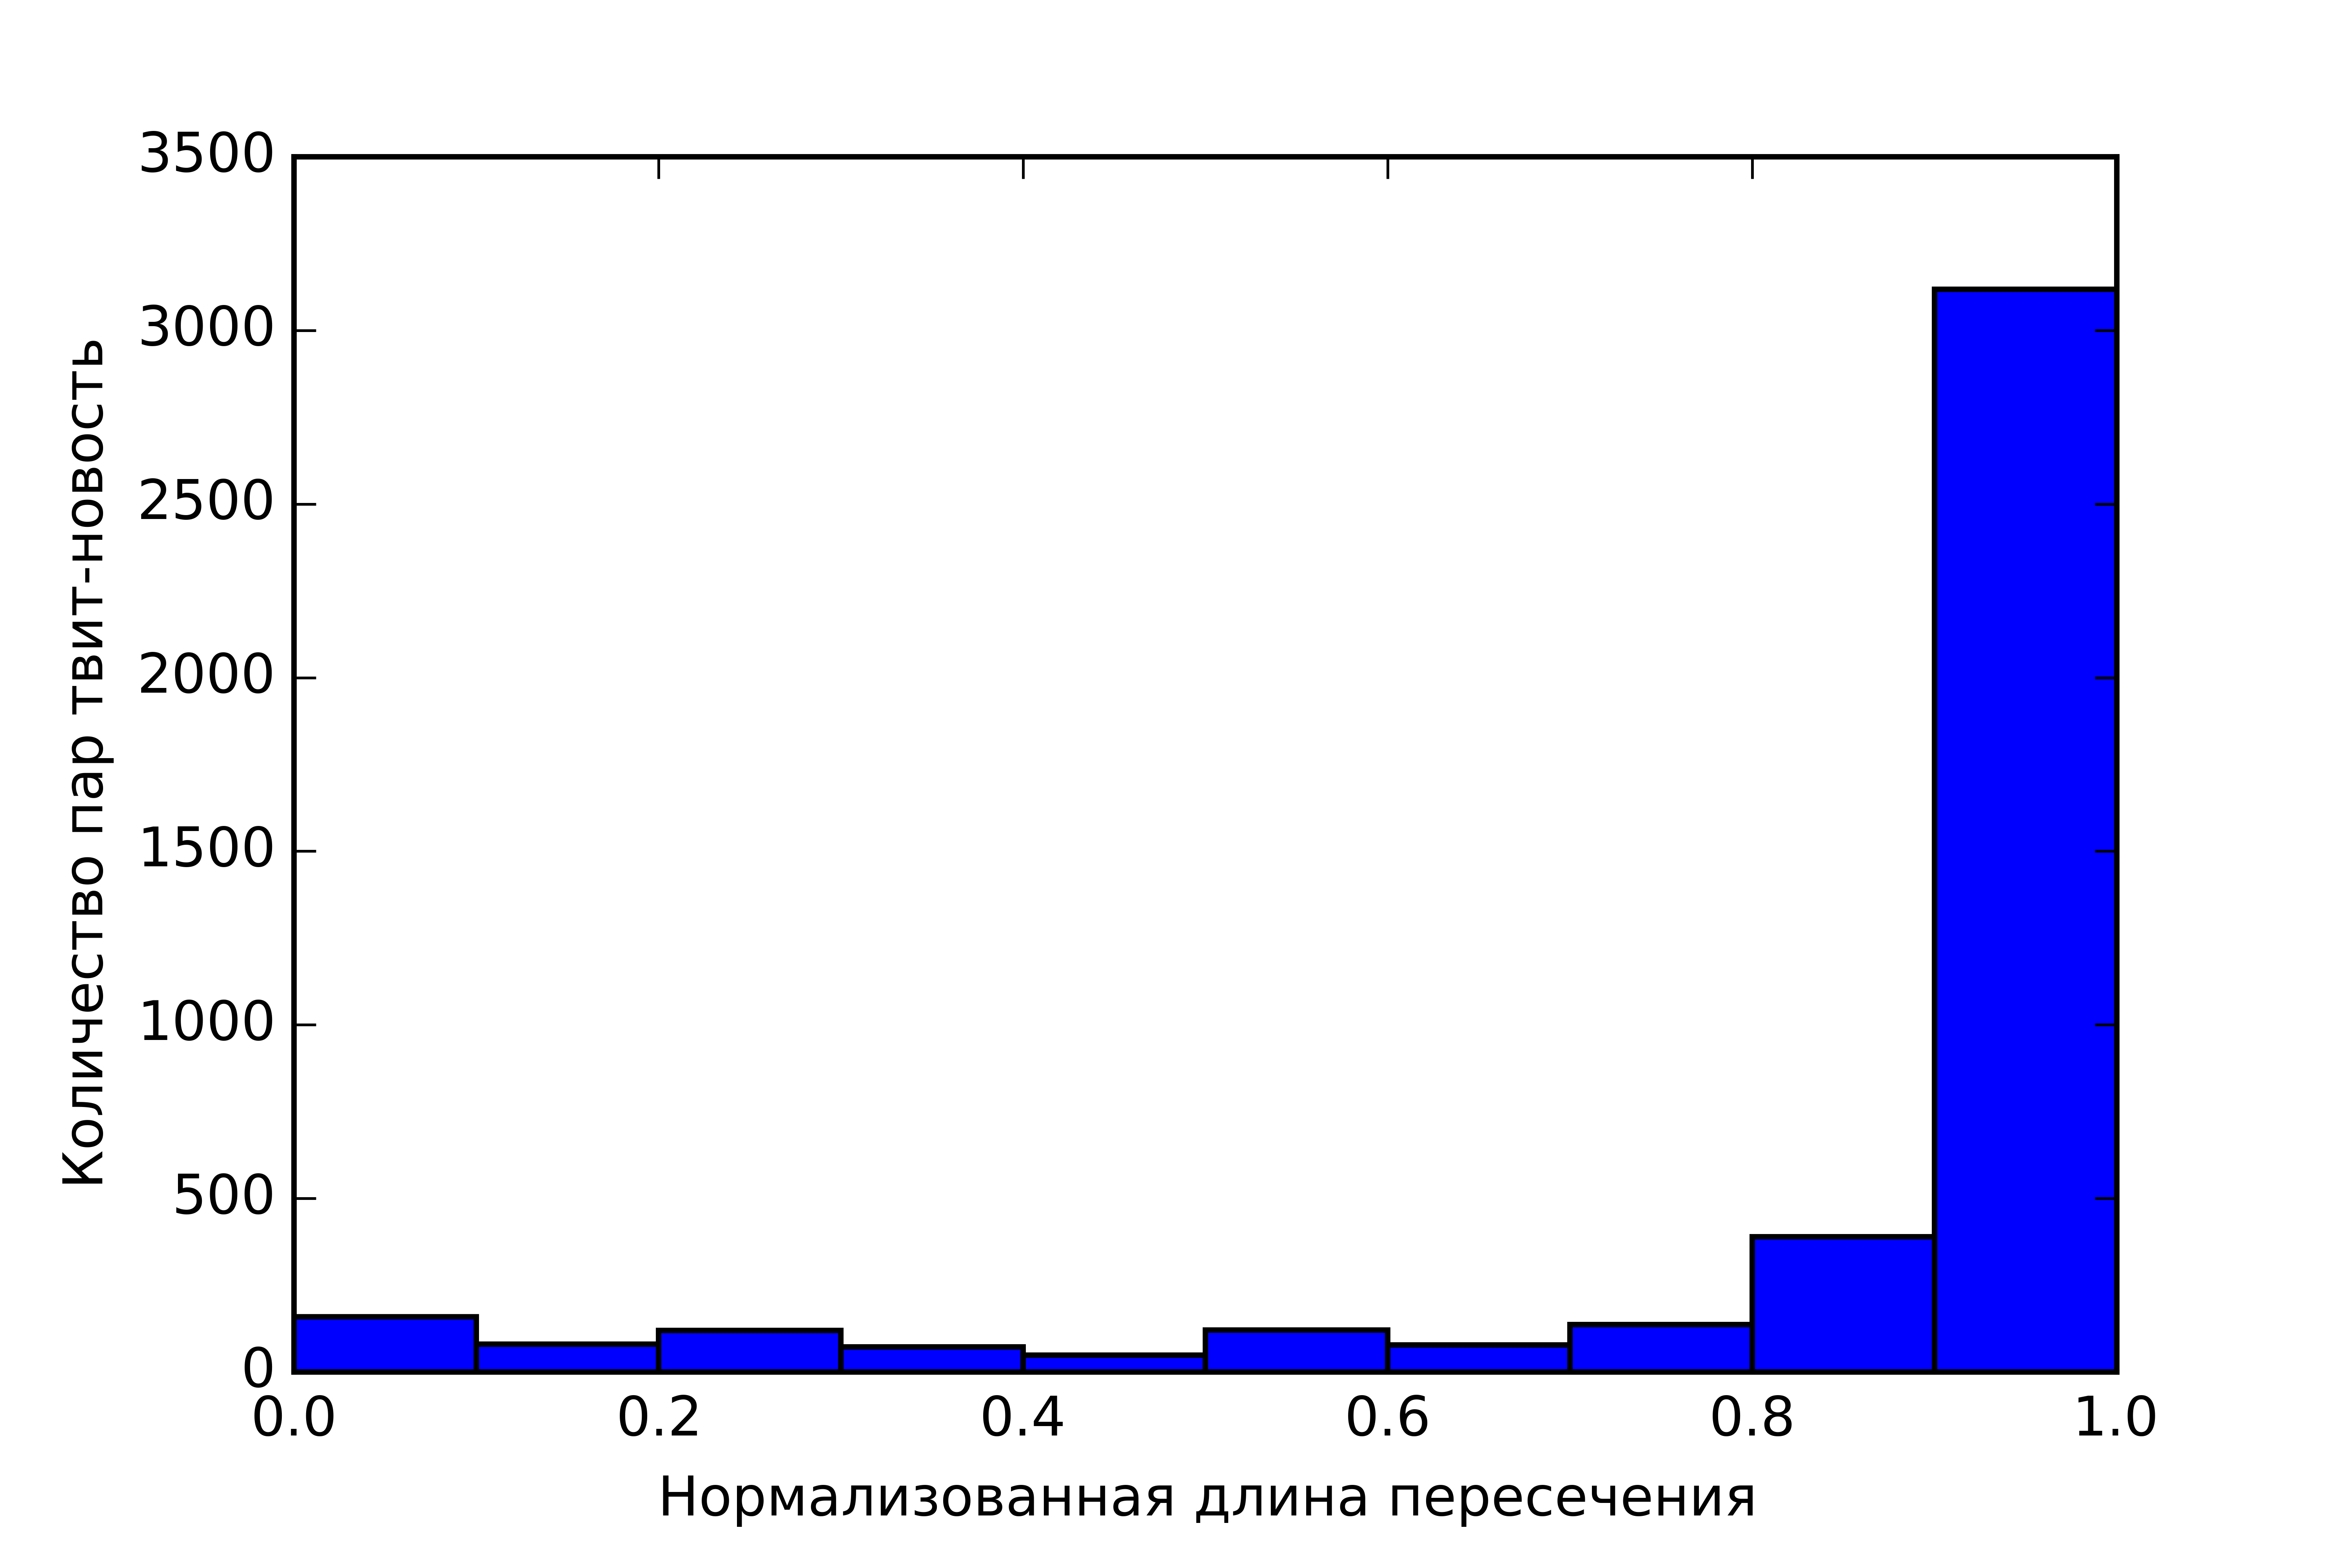
\includegraphics[scale=0.85]{dataset_auto_normalized_intersect_histogram.png}
            \caption{Зависимость количества пар твит-новости от нормализованный длины пересечения множеств слов (автоматически размеченный набор данных)}
            \label{pic:auto_histogram}
        \end{figure}
        Как видно из рисунка~\ref{pic:auto_histogram} слова в подавляющем большинстве твитов полностью совпадают со словами в соответствующей новости.
        Среди 4324 пар твит-новость в 3082 парах твит полностью совпадает с заголовком новости. Остаётся 1242 пар, которые не являются просто копией заголовка, среди этих пар
        нас интересуют те, в которых твит не является обрезанной частью заголовка статьи.

        Для выявления количества пар, где твит содержит информацию не содержащуюся в заголовке статьи посмотрим на зависимость количества пар твит-новость от процента уникальных слов в твите,
        эта зависимость изображена на рисунке~\ref{pic:auto_percent}.
        \begin{figure}[h!]
            \center
            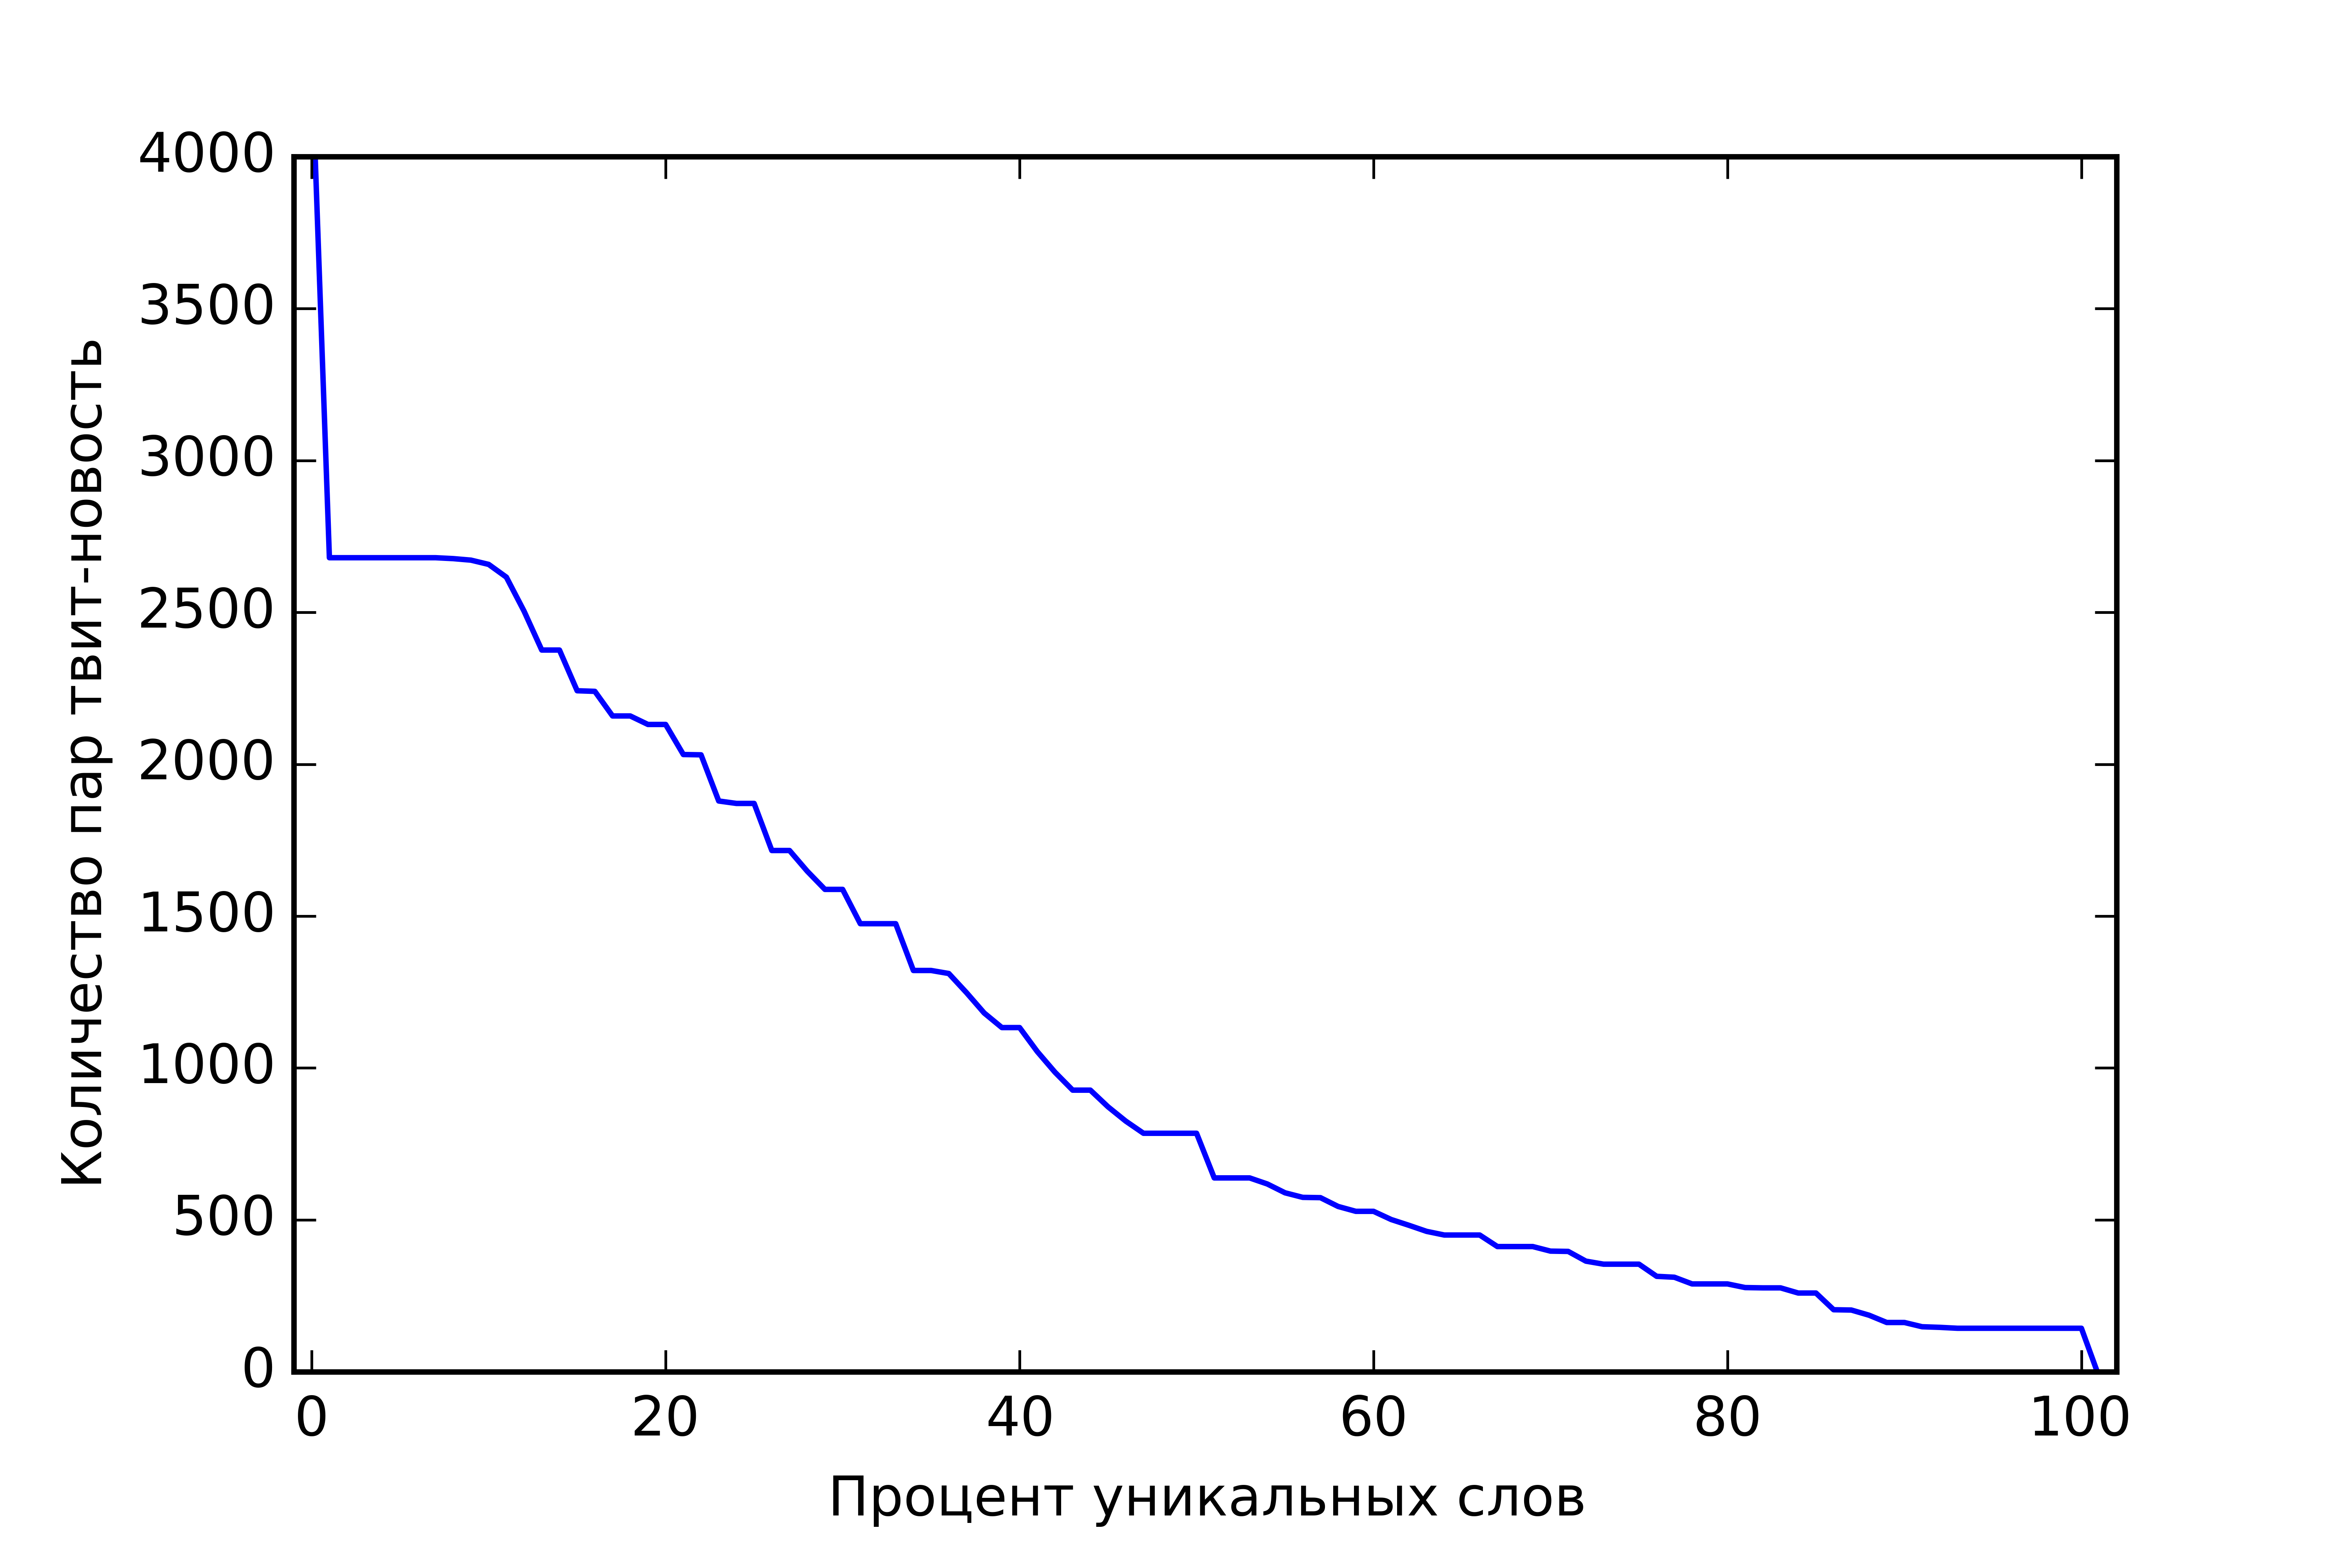
\includegraphics[scale=0.85]{dataset_auto_unique_words_percent.png}
            \caption{Зависимость количества пар твит-новости от процента уникальных слов в твите (автоматически размеченный набор данных)}
            \label{pic:auto_percent}
        \end{figure}
        Как видно из рисунка~\ref{pic:auto_percent} количество пар твит-новость, образующих нетривиальную связь, достаточно мало.

        На основе исследования зависимости можно получить грубую оценку количества нетривиальных связей.
        В исследуемом наборе данных таких связей порядка 500-1000, что очень мало и составляет примерно 12-23\% от общего числа пар.

    \subsubsection{Ручная разметка набор данных}
        Для получения большего количества нетривиальных пар твит-новость была предпринята ручная разметка набора данных.
        Для ручной разметки были предподготовлены данные. Основные этапы предподготовки данных:
        \begin{enumerate}
            \item на основе множества новостей строится список именованных сущностей $L$;
            \item случайным образом берётся подмножество $T$ множества твитов;
            \item из полученного множества $T$ удаляются все твиты, которые удолетворяют следующим правилам:
            \begin{enumerate}
                \item твит является ретвитом,
                \item твит содержит ссылку на URL с плохим доменным именем (под \textit{плохим доменным именем} подразумевается доменное имя,
                которое достаточно популярно и не ведёт на новостной источник, в работе использовался следующий список плохих доменных имён:\
                \url{apps.facebook.com}, \url{ask.fm}, \url{twitter.com}, \url{apps.facebook.com}, \url{www.instagram.com}, \url{vk.cc}),
                \item в приведённом к нормальной форме~(определение нормальной формы находится в главе~\ref{subsubsec:lemma}) тексте твита содержится менее 2 слов из списка именованных сущностей $L$;
            \end{enumerate}
            \item c помощью метода определения схожести текстов на основе частотности употребления слов каждому твиту сопоставляется 10 наиболее схожих с ним новостей.
        \end{enumerate}
        В качестве результата предподготовки получили множество пар твит-ранжированный список новостей.

        Предподготовленные данные были размечены.
        Разметка заключается в записи для каждого твита специальной отметки рядом с наиболее подходящей новостью из предложенного списка.
        Для каждого твита отмечалась только одна, наиболее подходящая новость, или не отмечалось ни одной.

        Было сформировано множество из 7373 пар твит-ранжированный список новостей. В нём было выявлено 1600 связей твит-новость.
        На основе размеченных вручную данных построен набор данных, состоящий из 1600 твитов, 13711 новостей, а также 1600 связей между ними.

        Для сравнения вручную построенного набора данных с набором данных, полученным автоматически, были построены две
        зависимости~---~зависимость количества пар твит-новость от длины пересечения слов твита и слов новости и зависимость количества пар твит-новости от процента уникальных слов в твите.
        На рисунке~\ref{pic:manual_histogram} изображена зависимость количества пар твит-новость от длины пересечения слов твита и слов новости, нормализованная по длине новости.
        \begin{figure}[h!]
            \center
            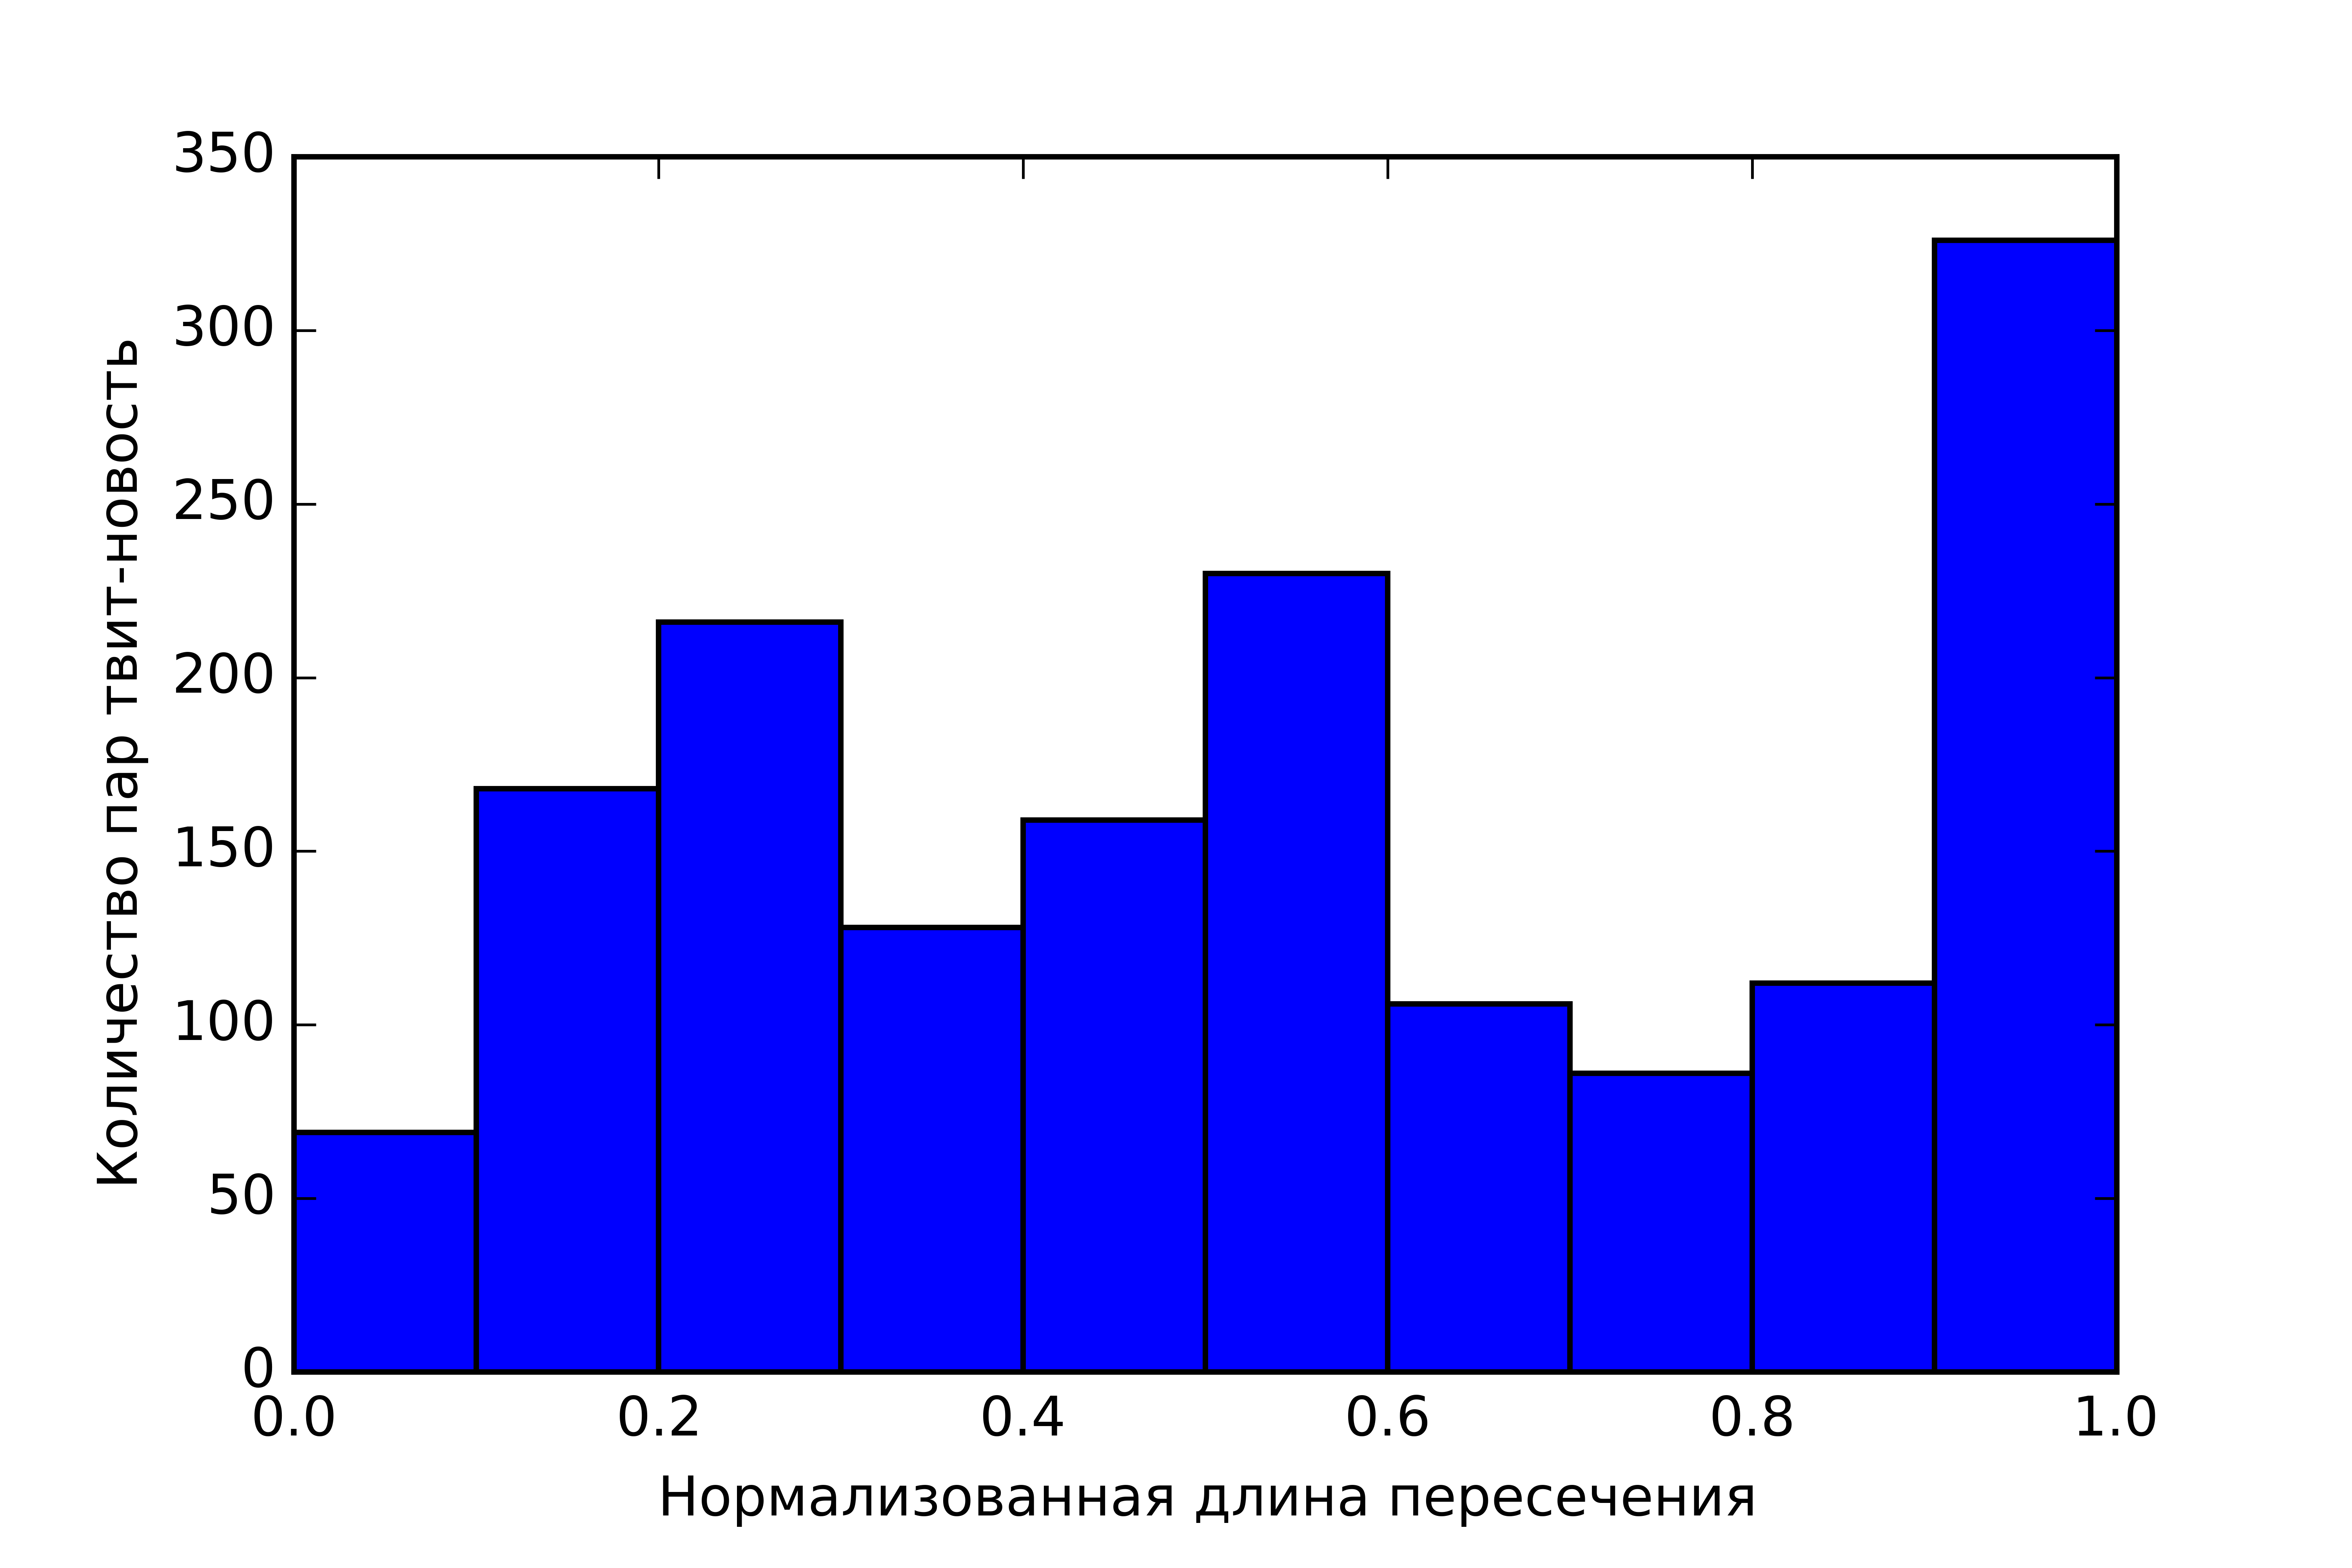
\includegraphics[scale=0.85]{dataset_manual_normalized_intersect_histogram.png}
            \caption{Зависимость количества пар твит-новости от нормализованный длины пересечения множеств слов (вручную размеченный набор данных)}
            \label{pic:manual_histogram}
        \end{figure}
        Как видно из рисунка~\ref{pic:manual_histogram} было получено распределение намного более близкое к равномерному, чем в случае автоматически размеченного набора данных.

        На рисунке~\ref{pic:manual_percent} изображена зависимость количества пар твит-новость от процента уникальных слов в твите.
        \begin{figure}[h!]
            \center
            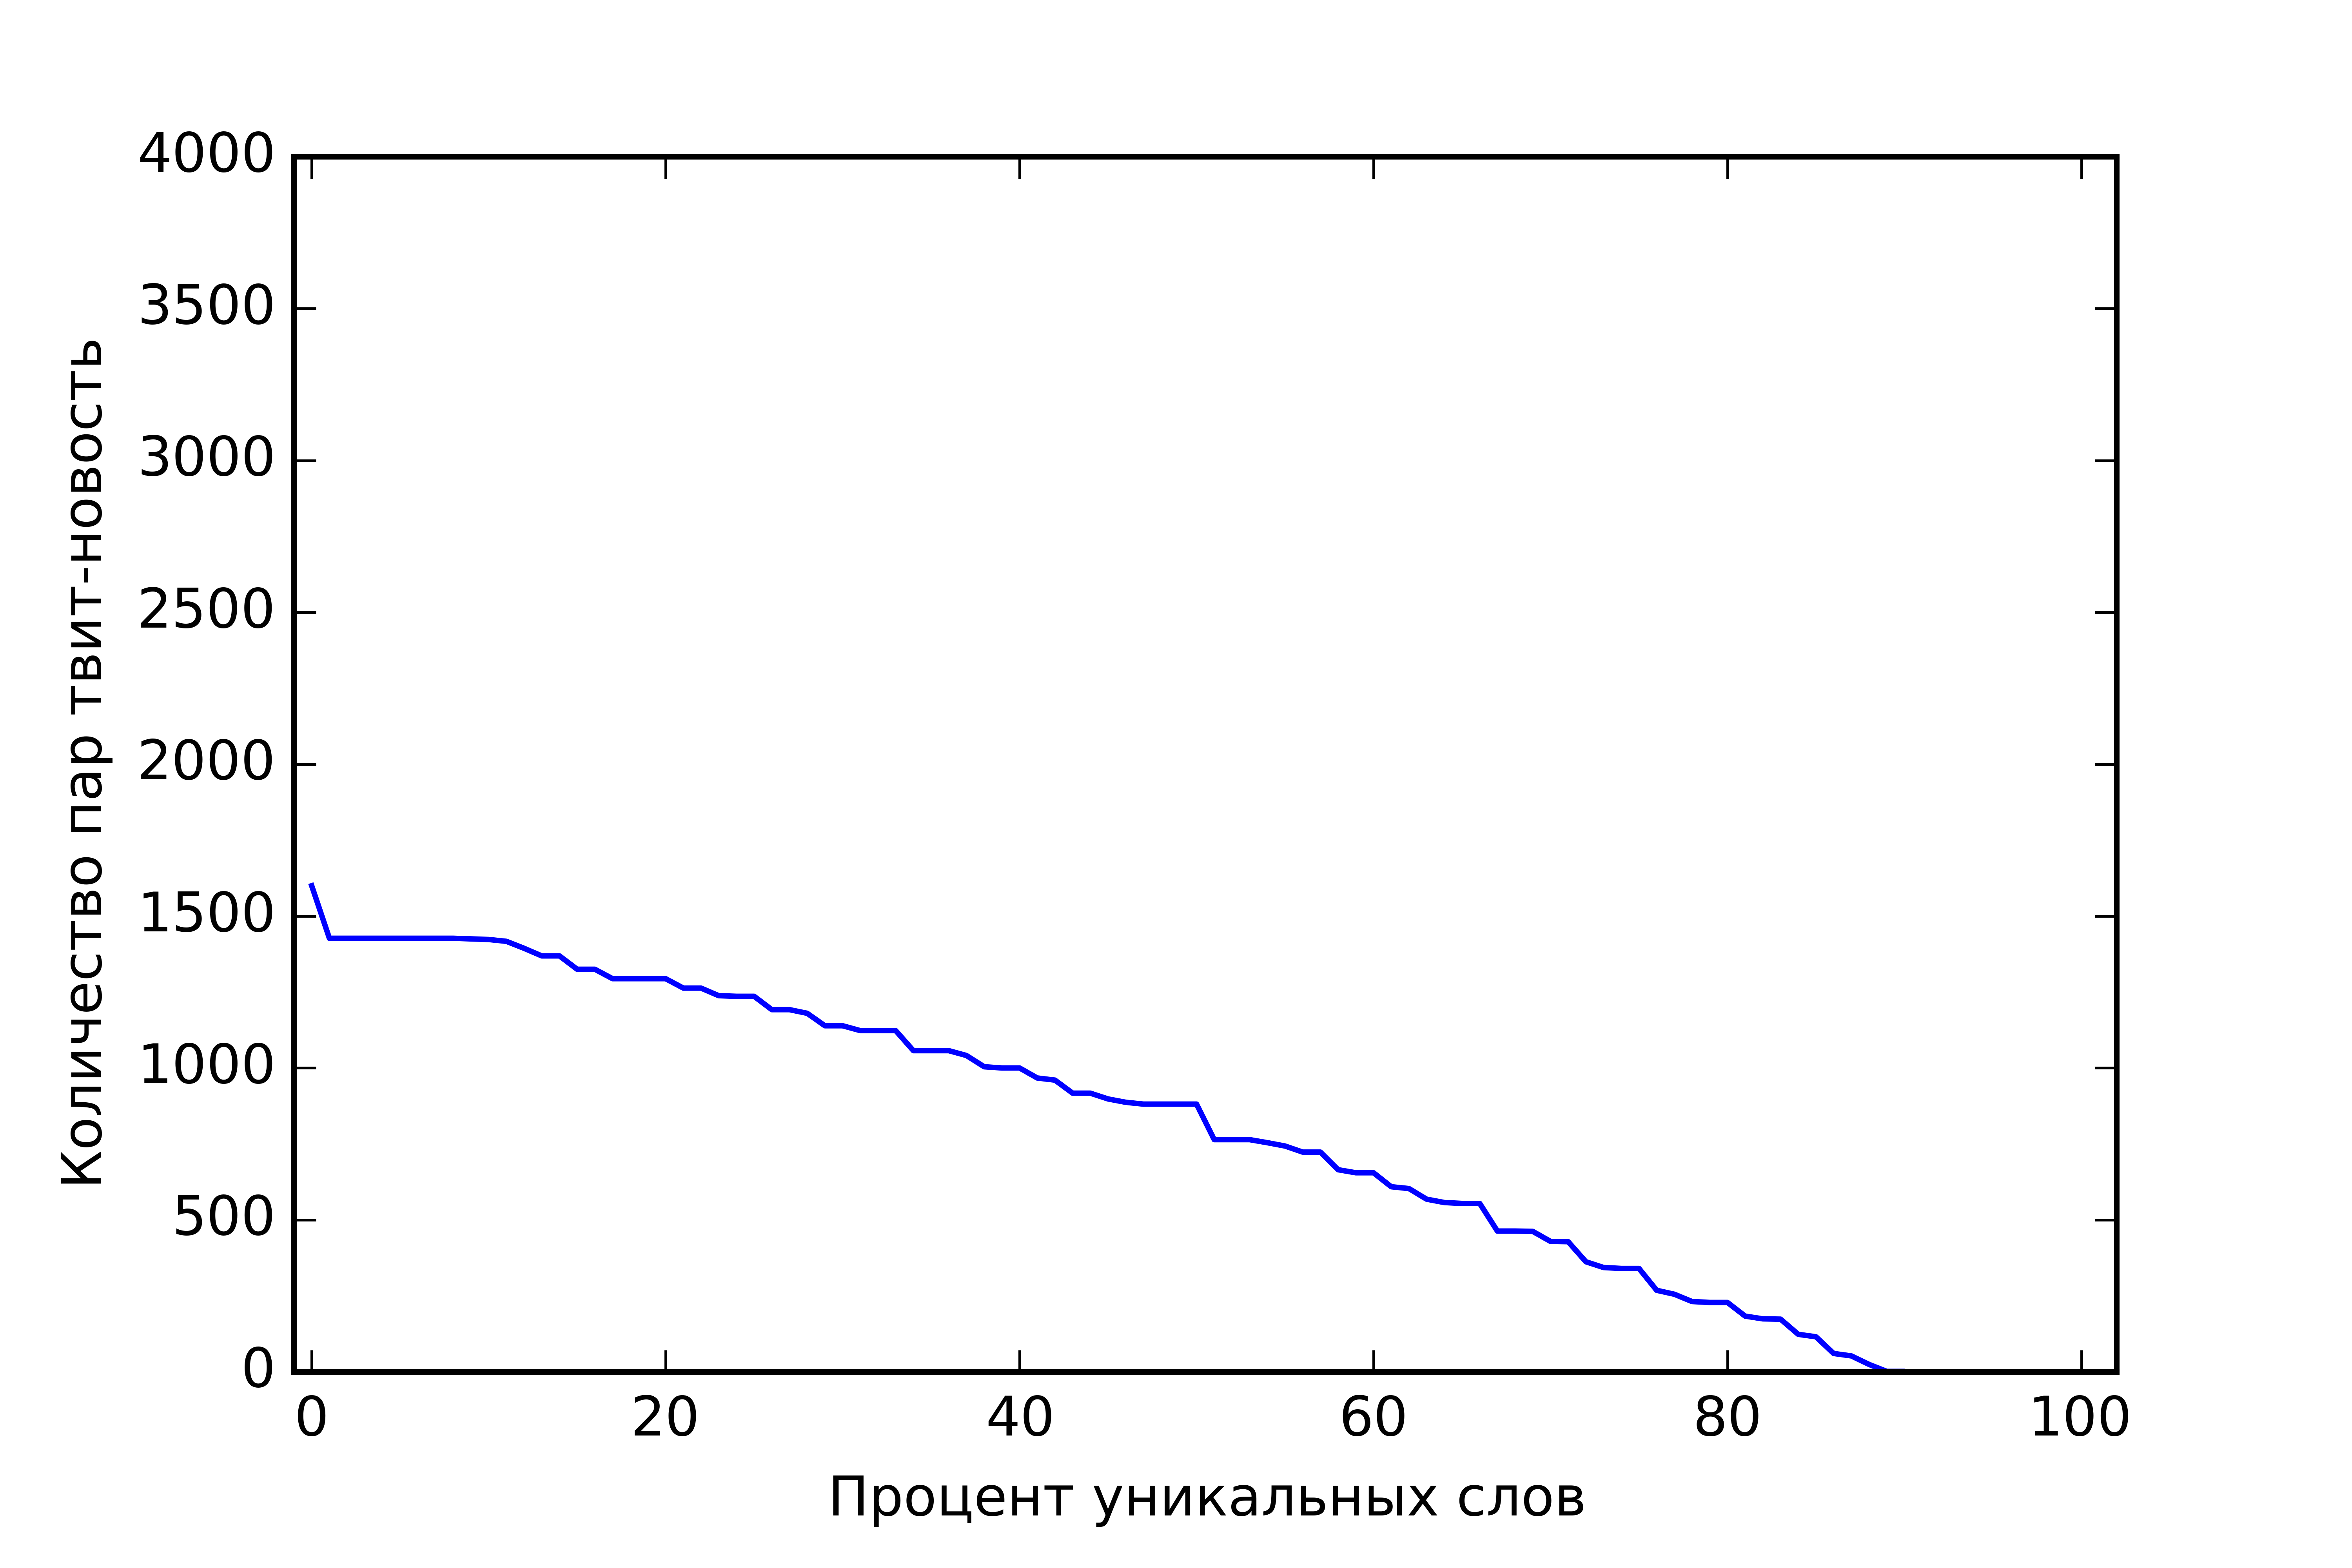
\includegraphics[scale=0.85]{dataset_manual_unique_words_percent.png}
            \caption{Зависимость количества пар твит-новости от процента уникальных слов в твите (вручную размеченный набор данных)}
            \label{pic:manual_percent}
        \end{figure}
        Как видно из рисунка~\ref{pic:manual_percent} количество твитов более с чем половиной уникальных слов сравнимо с аналогичным количеством в автоматически размеченном наборе данных,
        несмотря на то, что автоматически размеченный набор данных почти в три раза больше, чем вручную размеченный набор данных.
        Количественные значения полученных метрик приведены в таблице~\ref{tabular:dataset_stat}.

        \begin{table}[ht!]
            %\small
            \caption{Сравнение количества твитов \bigskip}
            \centering

            \label{tabular:dataset_stat}
            \begin{tabular}{|m{7cm}|c|c|}
                \hline
                \bf{\specialcell{Метрика}} &
                \bf{\specialcell{Автоматически \\ размеченный \\ набор данных}} &
                \bf{\specialcell{Вручную \\ размеченный \\ набор данных}} \\ \hline

                Количество связей & 4324 & 1600 \\ \hline
                Количество нетривиальных связей & 746 & 976 \\ \hline
                Процент нетривиальных связей от общего числа связей~(\%) & 17.25  & 61.00 \\ \hline
            \end{tabular}
        \end{table}
        Как видно из таблицы \ref{tabular:dataset_stat} вручную собранный набор данных намного более качественный, чем автоматический.
        Но как в ручном, так и в автоматическом наборе данных содержится очень мало нетривиальных связей твит-новость (в сравнении с количеством новостей).